Una vez elegidos los componentes y teniendo en cuenta los criterios de ruteo ya descriptos, se procedió al diseñó el circuito impreso mediante \textit{Orcad}. El primer paso es asignarle a cada componente su correspondiente \textit{footprint}, los cuales deben ser elegidos cuidadosamente y verificados por la hoja de datos. El diseño del circuito impreso se muestra en las Figuras \ref{fig.pcb_top} y \ref{fig.pcb_bottom}. 

\begin{figure}[H]
	\centering
	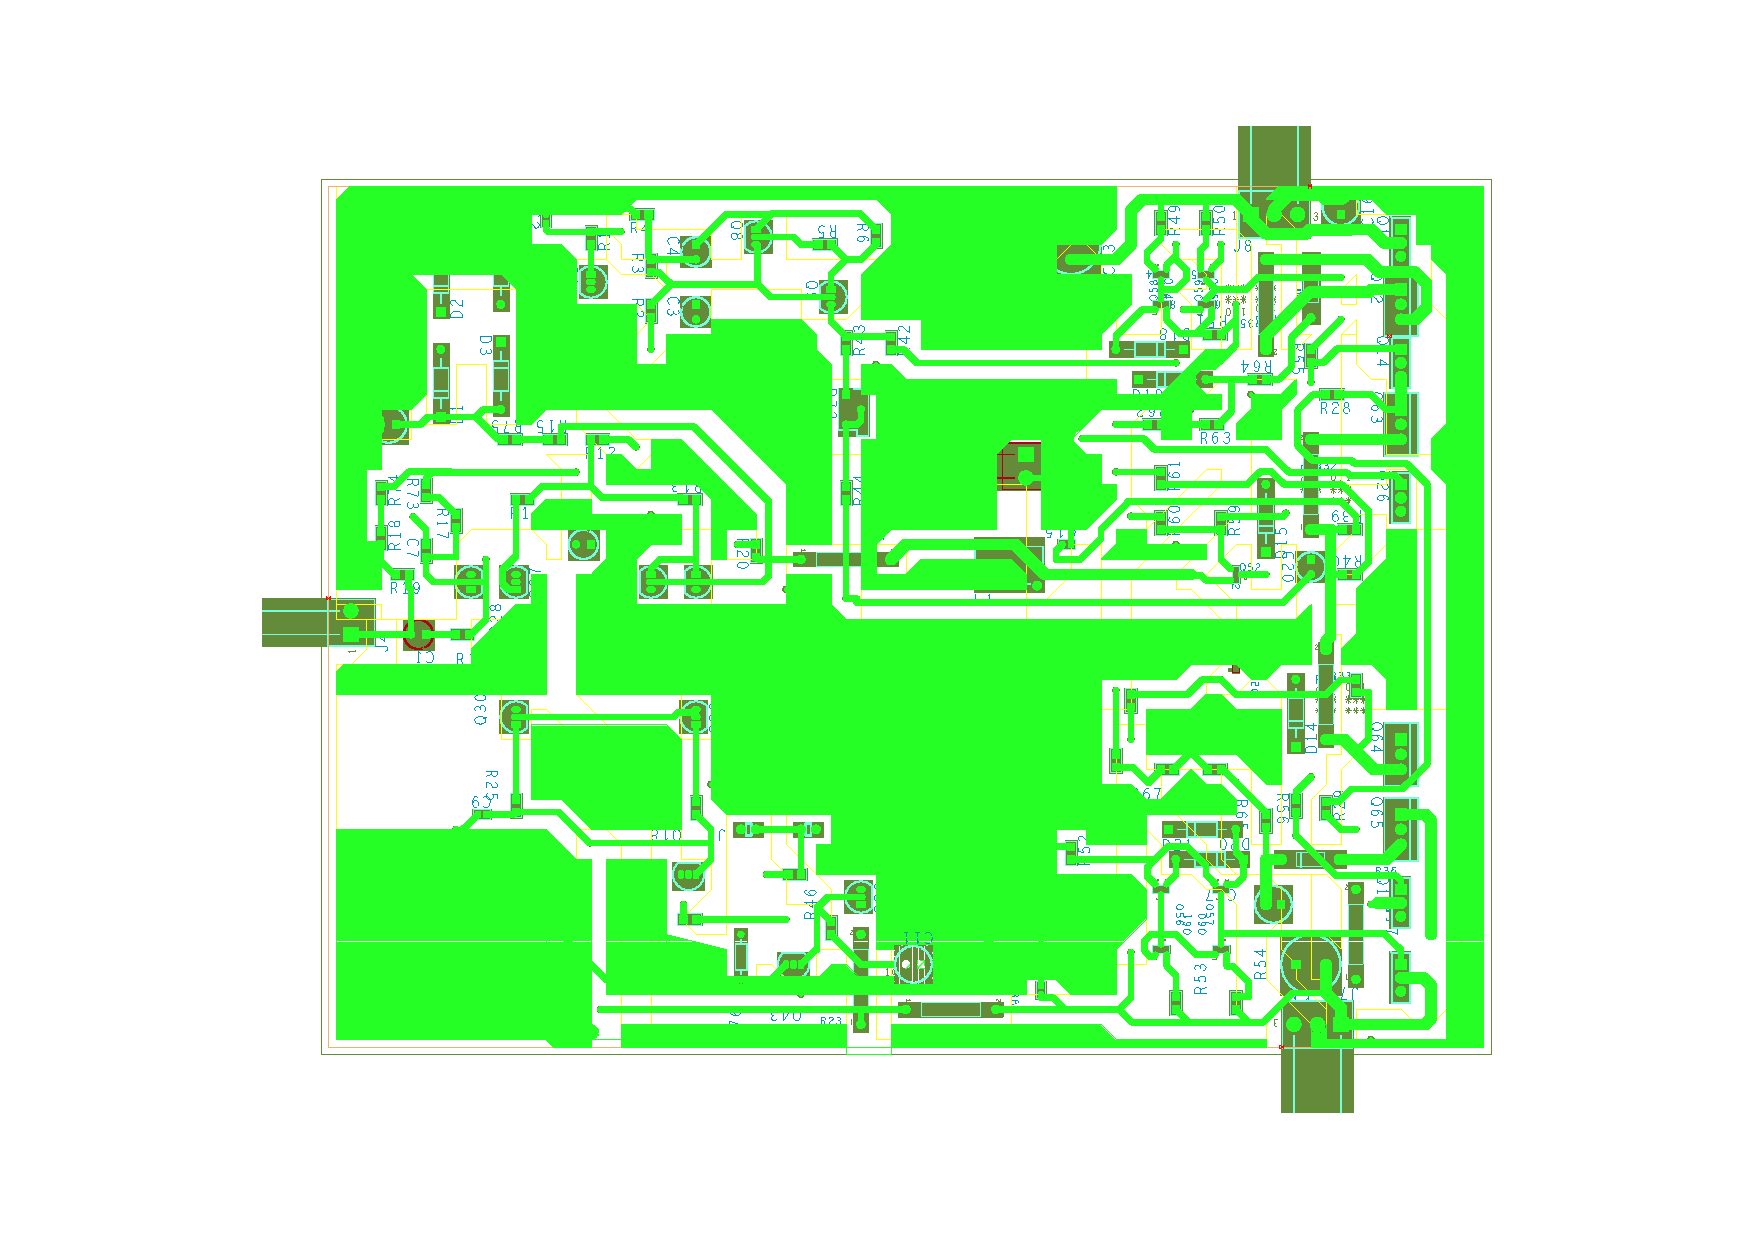
\includegraphics[width=0.8\textwidth, trim = 2cm 2cm 2cm 2cm]{top_color.pdf}
	\caption{Diseño de PCB, anverso.}
	\label{fig.pcb_top}
\end{figure}

\begin{figure}[H]
	\centering
	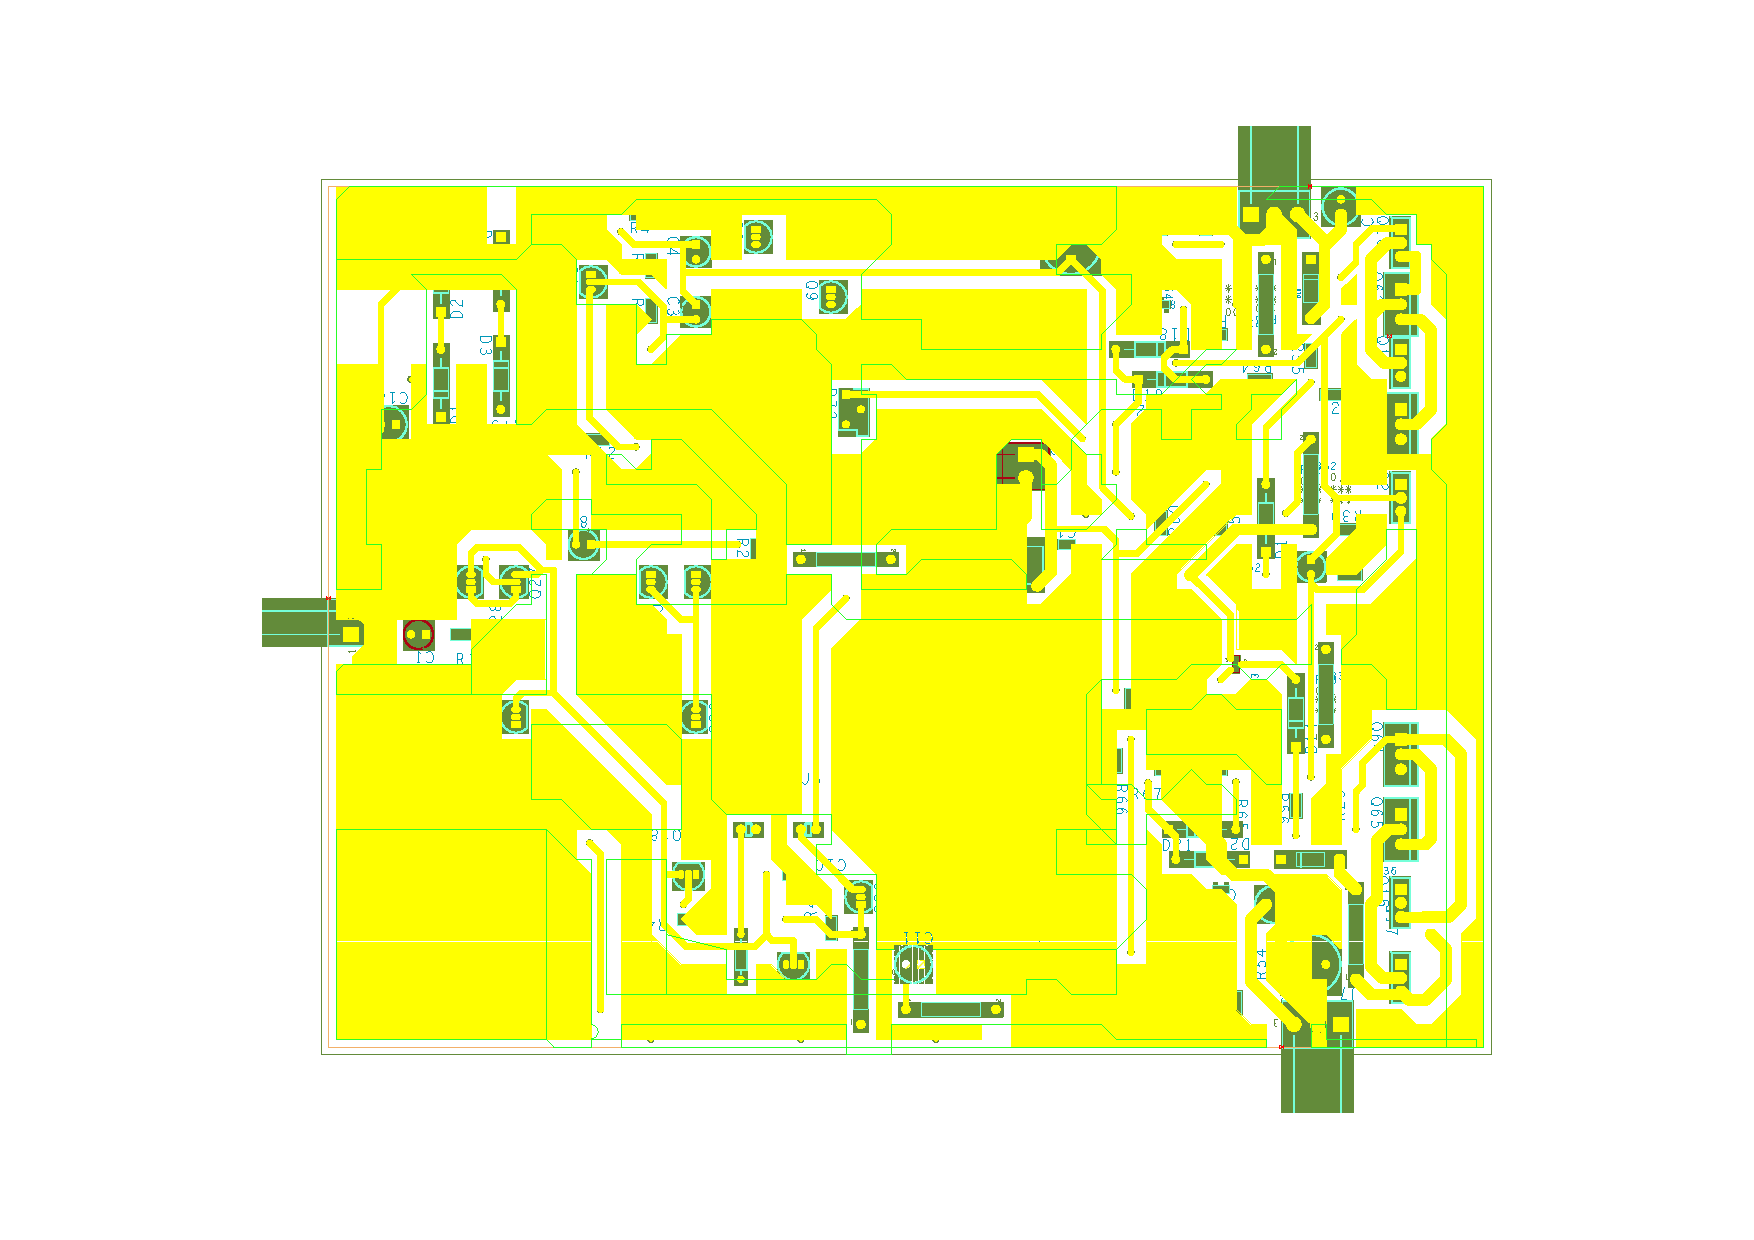
\includegraphics[width=0.8\textwidth, trim = 2cm 2cm 2cm 2cm]{bottom_color.pdf}
	\caption{Diseño de PCB, reverso.}
	\label{fig.pcb_bottom}
\end{figure}

%\HgraficarPNG{0.5}{top_color}{Diseño de PCB}{fig.pcb_top}
%\HgraficarPNG{0.5}{bottom_color}{Diseño de PCB}{fig.pcb_bottom}
